% -*- coding: utf-8 -*-
\documentclass[a4paper]{ctexart}
% \graphicspath{{Figures/}}
\usepackage{graphicx}             % 图片
\usepackage[colorlinks]{hyperref} % 使用超链接
\usepackage{booktabs}             % 表格
\usepackage{subfigure}            % 子图形
\graphicspath{{images/}}
\usepackage{amsmath}
\usepackage{amsfonts}

\title{工程结构优化}
\author{wyyjtu@gmail.com}
\date{\today}

\begin{document}
\maketitle

\section{问题}
如图 \ref{problem},已知 $P_1, P_2, P_3, P_4$ 四点的三维空间坐标和两个角度值 $\alpha, \beta$。求 $P_a, P_b$ 点的坐标,使 $P_a$ 和 $P_1, P_2$ 共线、$P_b$ 和 $P_3, P_4$ 共线,同时满足
$$\angle P_1P_aP_b = \alpha, \quad \angle P_aP_bP_4 = \beta.$$
\begin{figure}
  \centering
  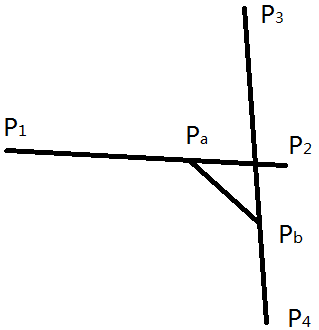
\includegraphics[width=0.4\textwidth]{problem.png}
  \caption{问题}
  \label{problem}
\end{figure}

\section{求解}
\subsection{问题分析}
由于求解 $P_a, P_b$ 的显式表达式非常复杂,而且还有多种情况,比如没有实数解、实数解在设计域以外等等。这里采用了工程结构优化设计方法,不仅可以找到设计域内满足要求的精确解,还能在没有精确解时找到设计域内最接近给定的 $\alpha, \beta$ 值的最优解。

两点 $P_a, P_b$ 之间的距离记为 $L_{ab}$,同理有 $L_{a1}, L_{b4}, L_{12}, L_{34}$。假设
$$m = \frac{L_{a1}}{L_{12}}, \quad n = \frac{L_{b4}}{L_{34}},$$
那么用两个设计变量 $m, n \in [0, 1]$ 就可以确定 $P_a, P_b$ 点的坐标
$$P_a = mP_2 + (1 - m)P_1, \quad P_b = nP_3 + (1 - n)P_4,$$
和 $\angle P_1P_aP_b, \angle P_aP_bP_4$ 的大小
$$\angle P_1P_aP_b = g(m, n) = arccos\left(\frac{\overrightarrow{P_aP_1} \cdot \overrightarrow{P_aP_b}}{\left|\overrightarrow{P_aP_1}\right| \left|\overrightarrow{P_aP_b}\right|}\right),$$
$$\angle P_aP_bP_4 = h(m, n) = arccos\left(\frac{\overrightarrow{P_bP_4} \cdot \overrightarrow{P_bP_a}}{\left|\overrightarrow{P_bP_4}\right| \left|\overrightarrow{P_bP_a}\right|}\right).$$

定义一个目标函数 $f(m, n)$ 来反应 $\angle P_1P_aP_b, \angle P_aP_bP_4$ 在任意点 $(m, n)$ 时和目标角度值 $\alpha, \beta$ 的偏差
$$f(m, n) = \sqrt{(\angle P_1P_aP_b - \alpha)^2 + (\angle P_aP_bP_4 - \beta)^2}.$$
这里的目标函数 $f(m, n)$ 也就是表征 $(m, n)$ 是不是最优设计点的评价指标。目标函数 $f(m, n)$ 的函数值越小,表示 $(m, n)$ 和要求的值越接近,最优解是目标函数取得最小值的点。$f(m, n)$ 的最小值分为以下两种情况:
\begin{itemize}
\item $f(m, n)_{min} = 0$,极值点是使 $\angle P_1P_aP_b, \angle P_aP_bP_4$ 等于 $\alpha, \beta$ 的解;
\item $f(m, n)_{min} > 0$,极值点不能使 $\angle P_1P_aP_b, \angle P_aP_bP_4$ 精确满足要求,而是在设计域内使角度值最接近 $\alpha, \beta$ 的解。
\end{itemize}

\subsection{结构优化问题}
结构优化问题可以提成:
\begin{flalign}
  \textrm{find} & \quad m, n & \\
  \textrm{min} & \quad f(m, n) & \\
  \textrm{s.t.} & \quad 0 \le m \le 1 & \label{eq:st1}\\
  & \quad 0 \le n \le 1 & \label{eq:st2}
\end{flalign}
也就是求最优的设计变量 $m, n$,使目标函数 $f(m, n)$ 最小,约束条件为方程 \ref{eq:st1},\ref{eq:st2}。

\subsection{优化结果}
在图 \ref{init} 所示的初始值下,目标函数 $f(m, n)$ 在 $m, n$ 的设计域 $[0, 1]$ 内分布情况如图 \ref{graph}。用序列二次规划算法求解,使目标函数取得最小值的最优解为:
\begin{verbatim}
When (m, n) = ( 0.723550421138,  0.223498396303):
f(m, n) = 0.000003

pa = (5287.716390, 55.289916, 1555.289916)
pb = (6055.300321, -738.956896, 1122.349840)

alpha = 134.999999
beta = 135.000003
\end{verbatim}
最优解对应的角度值,在误差允许范围内是满足工程需要的。

对不同的问题,可以在程序里修改图 \ref{init} 所示的初始值,用 MATLAB 重新计算。

\begin{figure}
  \begin{minipage}[t]{0.3\textwidth}
    \centering
    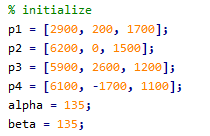
\includegraphics[width=\textwidth]{init.png}
    \caption{初始值}
    \label{init}
  \end{minipage}
  \begin{minipage}[t]{0.7\textwidth}
    \centering
    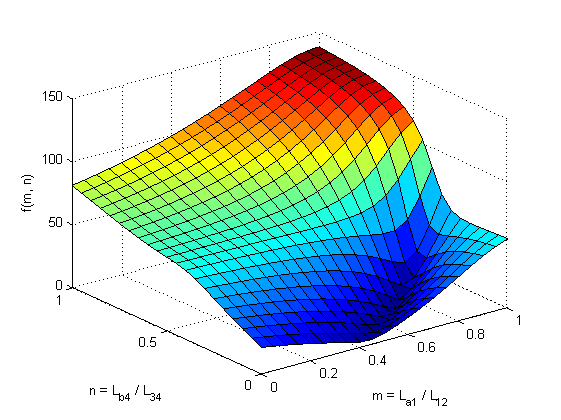
\includegraphics[width=\textwidth]{graph.png}
    \caption{目标函数}
    \label{graph}
  \end{minipage}
\end{figure}

\end{document}
